\begin{figure}[htbp]
\centering
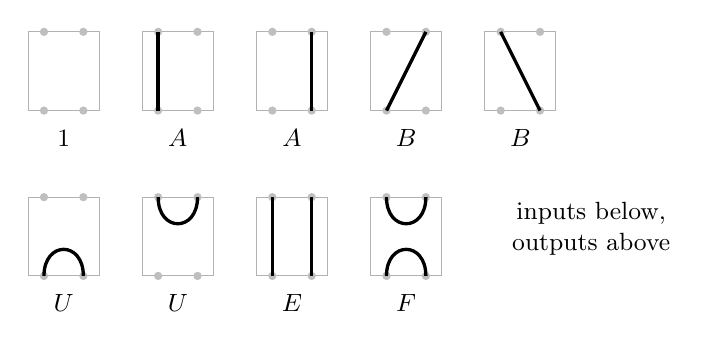
\begin{tikzpicture}[x=1cm,y=1cm,font=\small]
\foreach \j/\wt in {0/1,1/A,2/A,3/B,4/B,5/U,6/U,7/E,8/F}{
 \begin{scope}[xshift={1.45*mod(\j,5)*1cm},yshift={-2.1*floor(\j/5)*1cm}]
 \draw[black!30] (-.45,0) rectangle (.45,1);
 \foreach \x in {-.25,.25}{\fill[black!25] (\x,0) circle (1.5pt);\fill[black!25] (\x,1) circle (1.5pt);}
 \ifnum\j=1 \draw[very thick] (-.25,0)--(-.25,1);\fi
 \ifnum\j=2 \draw[very thick] (.25,0)--(.25,1);\fi
 \ifnum\j=3 \draw[very thick] (-.25,0)--(.25,1);\fi
 \ifnum\j=4 \draw[very thick] (.25,0)--(-.25,1);\fi
 \ifnum\j=5 \draw[very thick] (-.25,0) .. controls (-.25,.45) and (.25,.45) .. (.25,0);\fi
 \ifnum\j=6 \draw[very thick] (-.25,1) .. controls (-.25,.55) and (.25,.55) .. (.25,1);\fi
 \ifnum\j=7 \draw[very thick] (-.25,0)--(-.25,1) (.25,0)--(.25,1);\fi
 \ifnum\j=8 \draw[very thick] (-.25,0) .. controls (-.25,.45) and (.25,.45) .. (.25,0);\draw[very thick] (-.25,1) .. controls (-.25,.55) and (.25,.55) .. (.25,1);\fi
 \node at (0,-.35) {$\wt$};
 \end{scope}
}
\node[align=center] at (6.7,-1.5) {inputs below,\\outputs above};
\end{tikzpicture}
\caption{The nine local diagrams of $R(v)$, with coefficients evaluated
at $v$. Grey dots mark available slots; a slot is occupied exactly when a
black strand meets it. Gluing requires matching occupancies and assigns
zero to every closed component. These are operator diagrams, rather than
a geometric drawing of a rhombus.}
\label{fig:local-operator}
\end{figure}
